%! Author = Philipp Emmenegger
%! Date = 13/07/2021

\section{ASP.NET CORE}
\textbf{Weshalb:} Enterprise Framework, Kompilierbare Sprache (C\#), Komplett neue Entwicklung, Lauf auf allen Betriebssystemen.
\textbf{Convention over Configuration}.

\subsection{C\#}
\lstset[style=sharpc]
\begin{lstlisting}
// Anonyme Typen
var v =  new { Amount = 100, Message = "Arsch" }
// keine Typechecks / IntelliSense
dynamic person = new ExpandoObject();
// Extesion Methods
public static class MyExtensions {
    public static int WordCount(this string str) {
        return str.Split(new char[] {' ', '.'}).length;
    }
}
\end{lstlisting}

\subsection{Middleware}
\begin{lstlisting}
// Register Middleware
app.Use(async (context, next) => {
    System.Diagnostics.Debug.WriteLine("go req");
    await next.Invoke();
    System.Diagnostics.Debug.WriteLine("end");
});
// Verzweigung für Pfad erzeugen
app.Map("/logging", builder => {
    builder.Run(async (context) => {
        await context.ResponseWriteAsync("Arsch");
    });
});
// Request terminieren, keine neue Middleware
app.Run(async (context) => {
    await context.Response.WriteAsync("Yo");
});
\end{lstlisting}

\subsection{Dependency Injection}
ASP.NET kommt mit einem primitiven DI Container.\\
\textbf{Idee:} Klasse erwähnt welche Interfaces benötigt werden.
Ein Resolver sucht im Container nach einer geeigneten Klasse und übergibt diese.\\
\textbf{DI - Registrierung}
\begin{lstlisting}
public class Startup {
    // called by runtime, Used to add services
    public void ConfigureServices(IserviceCollection services) {
        services.AddTransient<IUserService, UserService>();
    }
    // Called by runtime, Configure HTTP req pipeline
    public void Configure(IApplicationBuilder app, IHostingEnvironment env, ILoggerFactory loggerFactory) {
        app.UseMiddleware<UserMiddleware>();
    }
}
\end{lstlisting}
\textbf{DI - Nutzen}
\begin{lstlisting}
public class UserMiddleware {
    private readonly RequestDelegate _next;
    // Captive Dependency*
    public UserMiddleware(RequestDelegate next, IUserService userService) {
        _next = next;
    }
    // No Captive Dependency
    public async Task Invoke(HttpContext context, IUserService userService) {
        await context.Response.WriteAsync(string.Join(", ", userService.Users));
    }
}
    //
\end{lstlisting}
\subsubsection{Lifetime}
\textbf{Transient:} Created each time they are requested.
Works best for lightweight, stateless services.\\
\textbf{Scoped:} Created once per request.\\
\textbf{Singleton:} Created the first time they are requested.
Every subsequent request will use the same instance.\\
\subsubsection{Captive Dependency}
Komponenten dürfen sich nur Komponenten mit gleicher oder längerer Lebensdauer Injecten lassen.

\subsection{Projekt-Struktur}
\textbf{wwwroot:} Statische Inhalte der Webseite (CSS / JS / HTML).
\textbf{appsettings.json:} Einstellungen der Webseite (Connection-String für DB).
\textbf{Programm.cs:} Einstiegspunkt der WebApp.
\textbf{Startup.cs:} Konfiguriert die WebApp.

\subsection{Razor}
\begin{lstlisting}
@{  var name = "John Doe"; 
    var weekDay = DateTime.Now.DayOfWeek; }
<p>Hello @name, today is @weekDay</p>
\end{lstlisting}

\subsubsection{Wichtige Dateien}
\textbf{Shared/\_layout.cshtml:} Generelles layout der App.
Definiert Sections (Placeholders), welche von der Page gefüllt werden.\\
\textbf{\_Layout.cshtml:} Struktur der Webseite, identisch für jede Seite.
\begin{lstlisting}
@RenderBody() // Platz für Content
@RenderSection("Nav", false); // Platz für Section
@section Nav{ /* ... */ }
\end{lstlisting}
\textbf{\_ViewStart.cshtml:} Hierarchisch, Code welcher vor den Razor-Files ausgeführt wird.
Definiert z.B. das Layout für alle Pages
\begin{lstlisting}
@{ Layout = "_Layout"; }
\end{lstlisting}
\textbf{\_ViewImports.cshtml:} Hierarchisch, Namespaces / Tag-Helpers können in diesem File registriert werden.

\subsubsection{Tag Helpers}
Ermöglichen C\# Code an HTML Tags zu binden.
Bsp: Email-Tag durch Link Tag ersetzen.
\begin{lstlisting}
public class EmailTagHelper : TagHelper {
    public string MailFor { get; set; }
    public override void Process(TagHelperContext context, TagHelperOutput output) {
        output.TagName= "a";
        output.Attributes.SetAttribute("href", "mailto:" + MailFor);
        output.Content.SetContent(MailFor);
    }
}
// Helper im ViewImports-file registrieren
@addTagHelper *, Microsoft.AspNetCore.Mvc.TagHelpers
@addTagHelper *, DataBinding
\end{lstlisting}

\subsubsection{Partials}
Markup Files, verwendet innerhalb von anderen Markup Files. 
Bessere Aufteilbarkeit und Wiederverwendbarkeit.
\begin{lstlisting}
<partial name="_Card" for="Card1" />
<partial name="_Card" model="..." />
\end{lstlisting}

\subsubsection{View Components}
Mächtigere Variante von Partials. 
Beinhalten Logik, können Daten laden / auf bearbeiten.
Rendert ein Teil der Webseite.\\
\textbf{Unterschied zu Pages:} Rendern nur ein Teil der Seite.\\
\textbf{Location:} \textit{/ViewComponents}\\
Razor-File: \textit{Pages/Shared/Components/[ComponentName]/[ViewName]}
\begin{lstlisting}
public class ToDoList: ViewComponent {
    public string[] Todos { get; set; }
    public ToDoList() { /* ... */ }
    public IViewComponentResult Invoke() {
        // /Pages/Shared/Components/TodoList/Default
        return View(Todos);
    }
}
// Razor File
@Page
@{ ViewData["Title"] = "ViewComponent"; }
<vc:to-do-list></vc:to-do-list>
@await Component.InvokeAsync("ToDoList")
\end{lstlisting}

\subsubsection{ViewData / TempData}
Mit Attribut Gekennzeichnete Daten werden allen Razor-Files im Render-Baum übergeben.\\
\textbf{ViewData / ViewBag:} Daten an das \_Layout übergeben\\
\textbf{TempData:} Überlebt ein redirect, Cookie-Middleware nötig (default aktiv)

\subsection{Pages}
Alternative und vereinfachte Variante vom MVC.
Router muss nicht konfiguriert werden.
Best-Practices für Serverseitiges-Rendering.\\
\textbf{Kombination mit MVC:} Statische Seiten mit Pages, REST-API mit MVC.

\subsubsection{Routing}
WebApp generiert anhand der URL eine Antwort.
Bei einem Aufruf wird im Folder \textit{/pages/} nach einer Page gesucht und ausgeführt (\textbf{case insensitive}):\\
\textit{/add} \textrightarrow \textit{/pages/add.cshtml}

\subsubsection{MVVM}
\textbf{*.cshtml:} View mit Razor
\begin{lstlisting}
@page
@model HelloWorldModel
@{ ViewData["Title"] = "HelloWorld"; }
<h1>@Model.HelloWorld</h1>
\end{lstlisting}
\textbf{*.cshtml.cs:} View Model
\begin{lstlisting}
public class HelloWorldModel : PageModel {
    public string HelloWorld { get; set; }
    public void OnGet() {
        HelloWorld = "Hi World!";
    }
}
    //
\end{lstlisting}

\subsubsection{Model}
Pro HTTP-Verb kann im VM eine Funktion definiert werden, die davor aufgerufen wird (OnGet / OnPost etc.).\\
\textbf{Body und Query werden automatisch gemappt:} Parameter werden als Argumente übergeben.
\begin{lstlisting}
public void OnPost(string echoText, long times) {
    EchoText = echoText;
    Times = times;
}
// Param können als Klasse übernommen werden
public void OnPost(EchoModel data) {
    Data = data;
}
// Ohne kopieren der Properties
public class PostModel : PageModel {
    [BindProperty]
    public string EchoText { get; set; }
}
\end{lstlisting}

\subsubsection{View}
\textbf{@page}: Definiert das Razor-File als Page\\
\textbf{@page "/test/\{id?\}":} Überschreibt die Default-Routing-Informationen\\
\textbf{Zugriff auf Routing Parameter:}
\begin{lstlisting}
// Im Razor-File
@page "/test/{id:int?}"
<p>ID: @RouteData.Values["id"]</p>
// Im Model
public int Id { get; set; }
[BindProperty(SupportsGet = true, Name = "Id")]
public int Id2 { get; set; }
public void OnGet(int id) { Id = id; }
\end{lstlisting}

\subsection{AJAX}
\subsubsection{Handlers}
Pages können Actions als handler anbieten.\\
\textbf{Namenskonvention:} \textit{On[Method][Name]}
\begin{lstlisting}
public IActionResult OnPostEcho(strong echoText) {
    return this.Content(echoText);
}
\end{lstlisting}
\textbf{Zugriff:} \textit{[Method]: /[Page]?handler=[HandlerName]}\\
Bsp: POST auf \textit{/Ajax?handler=echo}\\
\textbf{Rückgabewerte (IActionResult)}
\begin{itemize}
    \item ContentResult: StringResult, JsonResult, EmptyResult
    \item Status: NotFoundResult, StatusCodeResult
    \item Redirects: RedirectToPage, RedirectToPagePermanent
    \item Hilfsmethoden: Page(), Partial(), Content()
\end{itemize}

\subsection{Entity Framework}
\textbf{Code First benötigt:} Type Discovery (Welche Klassen in die DB), Connection String, DbContext (Entry Point)\\
\textbf{Migration:} EF Core erlauft keine automatische Migrationen von Model Änderungen mehr.
Aktuell nur über Konsole: \textit{dotnet ef database update}
\subsubsection{Entity Konventionen}
\textbf{public [long/string] Id:} wird automatisch zum PK\\
\textbf{public virtual ApplicationUser Customer:} Als Navigation Property erkannt\\
\textbf{public [long/string] CustomerId:} Als FK für Customer Property erkannt\\
\subsubsection{Wichtige Attribute}
\textbf{[Required]:} NotNull in DB,
\textbf{[NotMapped]:} Nicht in DB geschrieben,
\textbf{[Key]:} Definiert den PK,
\textbf{[MaxLength(10)]:} Allokationsgrösse in DB

\subsection{Validierung}
\subsubsection{Schritt 1: Annotieren der Klassen}
\textbf{Mögliche Attribute:} [StringLength(60, MinimumLength = 3)], [RegularExpression(@"...")], [Required], [DataType(DataType.Date)].
Attribute sind kombinierbar.
\subsubsection{Schritt 2: Razor anpassen}
\textbf{Validation ins DOM einfügen:}
\begin{lstlisting}
<div asp-validation-summary="ModelOnly"></div>
<span asp-validation-for="Item.Name"></span>
\end{lstlisting}
\textbf{JQuery Validation einbinden:}
\begin{lstlisting}
@section Scripts {
    <script src=".../jquery.validate.js"></script>
    <script src=".../...unobtrusive.js"></script>
}
\end{lstlisting}

\subsubsection{Schritt 3: Serverseitige Validierung}
\begin{lstlisting}
[HttpPost]
public ActionResult Index(Order order) {
    if(ModelState.IsValid) {
        order.CustomerId = User.Identity.GetUserId();
        _db.Orders.Add(order);
        _db.SaveChanges();
        return View("OrderOk", order);
    } return BadRequest();
}
\end{lstlisting}

\subsection{Authentifizierung}
\textbf{ASP.NET Identity Features:} PW Stärke, User Validator, Lockout Mechanismus, 2Faktor Auth, Reset PW, OAuth\\
\textbf{ASP.NET Identity Klassen:}
\begin{itemize}
    \item UserManager<ApplicationUser>
    \item RoleManager<IdentityRole>
    \item IAuthorizationService: Validation von Policies
    \item SingInManager
\end{itemize}

\subsubsection{Aktivierung \& Konfiguration}
\textbf{Startup.cs:}
\begin{lstlisting}
services.AddDefaultIdentity<IdentityUser>() // DI
    .AddEntityFrameworkStores<ApplicationDbContext>()
    .AddDefaultTokenProviders();
app.UseIdentity(); // Middleware
// Einstellungen
services.AddDefaultIdentity<IdentityUser>( options => {
    options.Password.RequireDigit = false;
    options.Password.RequiredLength = 8;
}).AddRoles<IdentityRole>()
.AddEntityFrameworkStores<ApplicationDbContext>()
\end{lstlisting}

\subsubsection{Anwenden}
\textbf{Attribute:}\\
\textit{[Authorize]:} User muss authentifiziert sein (Controller/Actions)\\
\textit{[AllowAnonymous]:} Ausnahme für spezifische Action
\begin{lstlisting}
this.User // Eingeloggter User Typ: ClaimsPrincipal
// CRUD Operationen über ApplicationUsers von DI
var user = await _userManager.GetUserAsync(User);
var id = _userManager.GetUserId(User);
\end{lstlisting}
\textbf{Claim:} Statement über einen User, ausgestellt von einem Identity Provider.\\

\subsubsection{Authentifizierung Prüfen}
\begin{lstlisting}
// Automatisch
[Authorize]
public ActionResult Create() { return View(order); }
// Manuell
public ActionResult Create() {
    if(User.Identity.IsAuthenticated) { /* ... */ }
    else { return new StatusCodeResult(401); }
}
\end{lstlisting}

\subsection{Authorisierung}
\begin{lstlisting}
// Lösung 1: Attribute:
[Authorize(Roles = "Admin, PowerUser")]
[Authorize(Policy = "OlderThan18")]
// Lösung 2: Services:
var isInRole =
    await _userManager.IsInRoleAsync(user,"Admin");
// Lösung 3: Claims
User.HasClaim(ClaimTypes.Role, "Admin")
\end{lstlisting}

\subsubsection{Policy}
Ermöglichen es, komplexere Regeln zu definieren.
\begin{lstlisting}
options.AddPolicy("Founders", policy => {
    policy.RequireAuthenticatedUser();
    policy.RequireClaim(ClaimTypes.Name, "joe", "");
});
\end{lstlisting}

\subsubsection{Authorizierung mit Razor}
\begin{lstlisting}
@inject UserManager<ApplicationUser> manager;
@inject ApplicationDbContext context;
@{
    var user = await manager.GetUserAsync(User);
    if(user != null &&
        await manager.IsInRoleAsync(user, "Admin"))
        { /* ... */ }
}
\end{lstlisting}

\subsection{Testing}
\textbf{Unit Test mit ASP.NET}
\begin{lstlisting}
public class UnitTest {
    [Fact]
    public void TestName() { /* ... */ }
}
\end{lstlisting}

\subsection{App Secrets}
Ermöglicht es, Secrets in einem separaten File zu persistieren.
\begin{lstlisting}
// Wert setzen:
dotnet user-secrets set "admin-pwd" "123456"
// Wert nutzen:
if(env.IsDevelopment()) {
    builder.AddUserSecrets<Startup>(); }
app.ApplicationServices.GetService<DataService>()
    .EnsureData(Configuration["admin-pwd"]);
\end{lstlisting}

\subsection{API Routing}
\subsubsection{Startup}
Nur die nötigen Services und Endpoints registrieren.
\begin{lstlisting}
public void ConfigureServices(IServiceCollection services) {
    services.AddRazorPages();
    services.AddControllersWithViews();
    services.AddControllers();
    services.AddMvc();
}
public void Configure(IApplicationBuilder app,
                    IWebHostEnvironment evn) {
    app.UseRouting();
    app.UseEndpoints(endpoints => {
        endpoints.MapControllers();
        endpoints.MapRazorPages();
        endpoints.MapBlazorHub();
    });
}
\end{lstlisting}

\subsubsection{Verwendung}
Funktioniert über Attribute. \textit{[Route]} definiert einen neuen Eintrag im Router.
\textit{[HttpMethod]} bei Actions ist required.\\
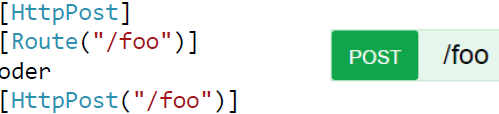
\includegraphics[width=0.45\linewidth]{img/asp_api_routing.png}
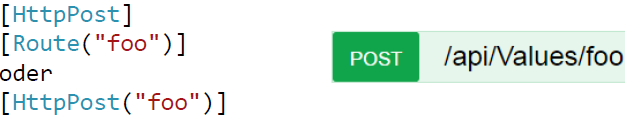
\includegraphics[width=0.55\linewidth]{img/asp_api_routing2.png}

\subsection{Swagger}
Eine Spezifikation für die Dokumentation von REST APIs.
Programmiersprachen unabhängig.
Wird im \textit{Startup.cs} eingetragen.
Defaultmässig unter \textit{http://[server-name]/swagger} erreichbar.
C\# ermöglicht es Kommentare als XML zu exportieren.
Dieses XML-File kann von Swagger genutzt werden um die API zu beschreiben.
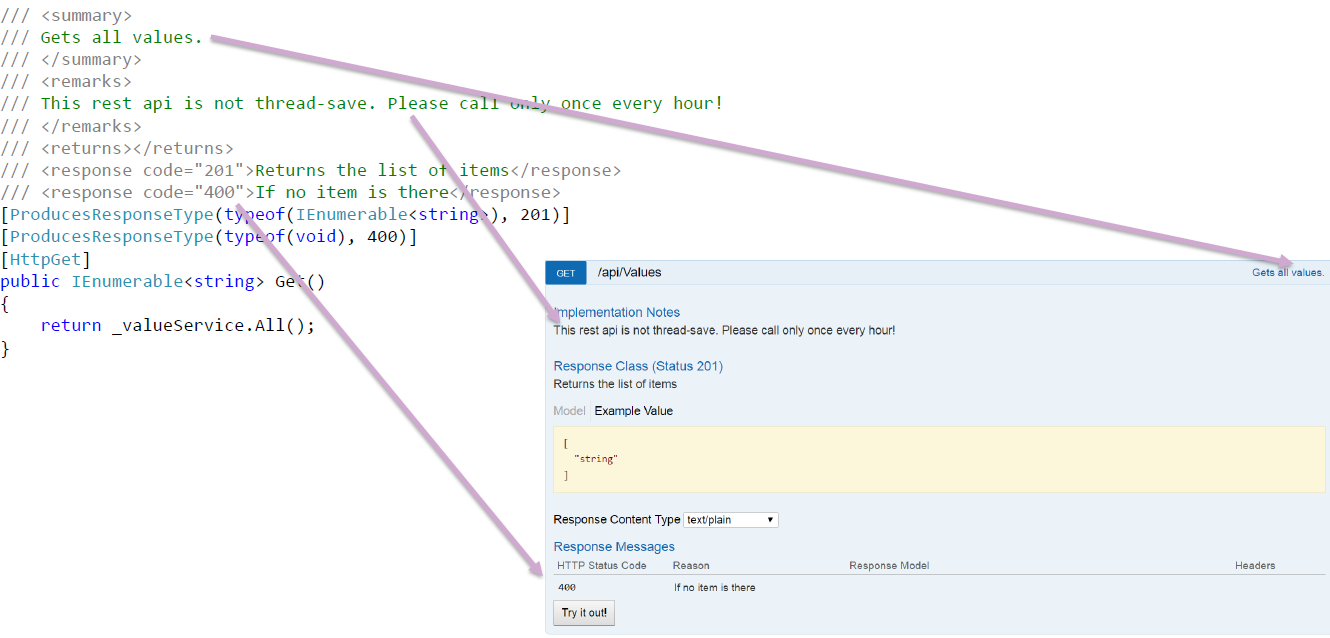
\includegraphics[width=\linewidth]{img/asp_swagger.png}

\subsection{REST HATEOAS}
\textbf{Idee:} Verlinkte Daten als Links zu Verfügung stellen.

\subsection{Exception Handling}
Error Handling soll generisch funktionieren.\\
\textbf{Vorgehen:} Es gibt eine Exception, welche die notwendigen Daten sammelt.
Es gibt einen globalen Errorhandler, welcher diese Exception für Client aufbereitet.
Bei einem ungültigen Zustand wird Custom-Exception ausgelöst.